\chapter{Tipos de dados Especiais}
Neste capítulo veremos alguns tipos de dados especiais que o MDArte implementa e
como utilizá-los, a fim de facilitar a comunicação com o banco de dados e o
tratamento dos dados da aplicação.

\section{Hstore}
O hstore é um tipo de dados disponível no Postgres que permite, para uma mesma
coluna de uma linha na tabela, relacionar valores de texto à chaves, que também
são textos, tal qual um Map em Java.
Para mais informações sobre o funcionamento do hstore, consulte
http://www.postgresql.org/docs/9.4/static/hstore.html.
Nesta seção veremos como utilizar o tipo hstore nas entitades de um sistema
desenvolvido com o MDArte.

\subsection{Criando um atributo com o tipo hstore}
No diagrama de classes da sua camada de domínio, abra a especificação do
atributo que deverá ser do tipo hstore. No campo type, selecione o tipo Hstore,
como na imagem abaixo:
\begin{figure}[H]
	\centering
	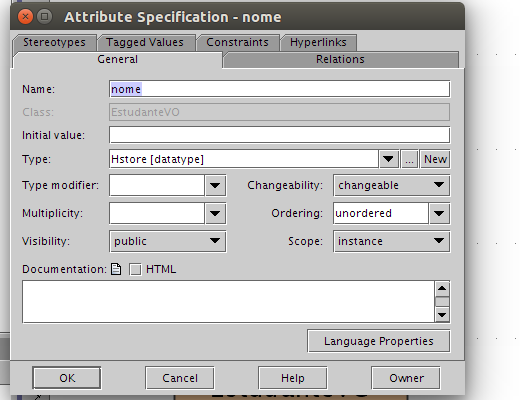
\includegraphics[width=290pt,height=220pt]{files/imgs/hstore-0000.png}
	\caption{Configuração do parâmetro matrícula da classe Estudante.}
	\label{config_parametro}
\end{figure}

O resultado na classe que representa a entidade, será o seguinte:
\begin{figure}[H]
	\centering
	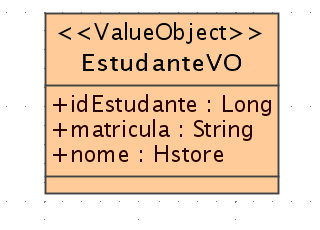
\includegraphics[width=260pt,height=180pt]{files/imgs/hstore-0001.png}
	\caption{Entidade com o atributo nome já com o tipo hstore.}
	\label{config_parametro}
\end{figure}

Feito isto, vá na pasta raiz do projeto e regere o mesmo usando o comando
\texttt{maven}. O \texttt{MDArte} irá então regerar as classes da camada de
domínio, bem como os \texttt{scripts SQL} corrspondentes aos novos atributos da
entidade. Você provavelmente precisará rodar novamente o \texttt{script
schema-create.sql}, ou alterar manualmente a tabela, a fim de que o atributo
escolhido como \texttt{hstore} tem a tipagem correta na tabela do banco. Você
provavelmente precisará também reinserir os dados da sua aplicação, caso a
tabela já tenha alguma informação.

\subsection{Acessando um atributo hstore}
Quando um atributo de uma entidade é modelado como sendo do tipo
\texttt{Hstore}, o \texttt{MDArte} o mapeará para o código da aplicação como um
\texttt{Map}, mais especificamente um \texttt{HashMap}. Como resultado disso, o
atributo será gerado nas classes de \texttt{<nomeDaEntidade>TO} e
\texttt{<nomeDaEntidade>Abstract} com o tipo \texttt{Map}.

Para acessar e alterar os valores do \texttt{Map} são gerados os seguintes
métodos:

\texttt{public void set<nomeDoAtributo>(String key, String value)} - Adiciona um
novo valor no indice indicado.

\texttt{public void set<nomeDoAtributo>(Map<String,String> map)} - Substitui o
\texttt{map} da entidade por um \texttt{clone} do \texttt{map} passado por
parâmetro.

\texttt{public String get<nomeDoAtributo>(String key)} - Retorna o valor do
\texttt{map} correspondente à chave passada por parâmetro.

\texttt{public Map<String,String> get<nomeDoAtributo>()} - Retorna um
\texttt{clone} do \texttt{map} existente na classe da entidade.

\texttt{public void remove<nomeDoAtributo>(String key)} - Remove do \texttt{map}
a chave correspondente \texttt{string} passada por parâmetro.

\subsection{Hstore e persistência de dados}
A persistência dos dados com o \texttt{Hstore} é bem parecida com a dos demais
atributos, todas as alterações feitas nos indíces do \texttt{map} serão
persistidas mediante o uso dos métodos \texttt{update} ou \texttt{insert} na 
classe de serviço da entidade. No entanto, a filtragem de dados baseada no
atributo \texttt{Hstore} não está disponível, ou seja, sempre que executada uma
filtragem de dados em uma entidade, caso haja um atributo do tipo
\texttt{Hstore}, os valores do mesmo serão desconsiderados na operação.

\section{\texttt{JSONB}}
O \texttt{JSONB} é um tipo de dados suportado pelo \texttt{Postgres} a partir da
versão 9.4, permitindo salvar dados no formato \texttt{JSON} com diversas
facilidades e possibilidade de filtrar dados usando os dados contidos na coluna
de tipo \texttt{JSONB}.

Nesta seção, veremos como utilizar o suporte do \texttt{MDArte} a este tipo de
dados especial. 

É importante ter em mente que no \texttt{MDArte} o \texttt{JSONB} é utilizado
como uma forma de modelar uma \texttt{'subentidade'}, um conjunto de
informações, em json, que só fazem sentido em conjunto, formando uma espécie de
entidade, só que não precisando ter um \texttt{id} ou tabela próprios para si,
podendo ser um campo de outra entidade.

\subsection{Modelando uma subentidade \texttt{JSONB}}
Agora veremos como modelar uma subentidade \texttt{JSONB} no \texttt{MDArte}.
Usaremos como exemplo o modelo de \texttt{Camada de Domínio} do \texttt{Sistema
Acadêmico}. O modelo começará da seguinte forma:

\begin{figure}[H]
	\centering
	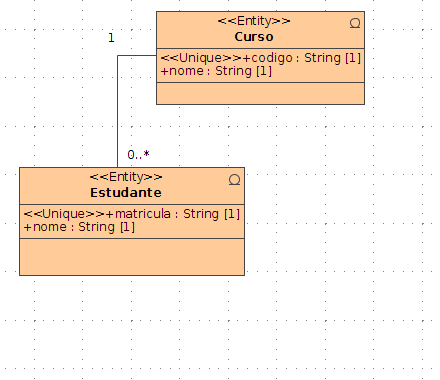
\includegraphics[width=290pt,height=240pt]{files/imgs/tutorial-mdarte-jsonb-0004.png}
	\caption{Modelo inicial da camada de domínio.}
	\label{camada_dominio}
\end{figure}

Começaremos criando uma nova classe no diagrama. A título de exemplo, criaremos
uma classe de nome \texttt{Endereco}. Adicionaremos também alguns campos a ela.
O diagrama ficará da seguinte forma:

\begin{figure}[H]
	\centering
	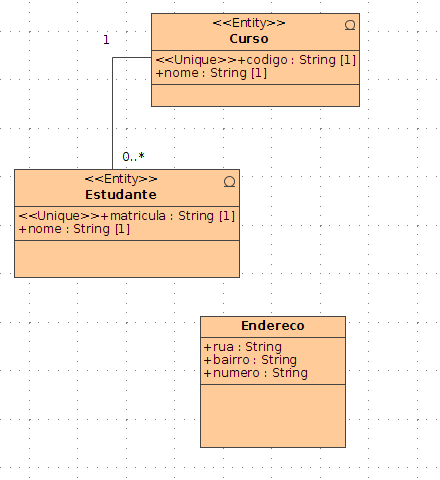
\includegraphics[width=290pt,height=280pt]{files/imgs/tutorial-mdarte-jsonb-0003.png}
	\caption{Camada de domínio já com a classe Endereco.}
	\label{camada_dominio_endereco}
\end{figure}

Em seguida, marcaremos a classe \texttt{Endereco} com os estereótipos
\texttt{«Entity»} e \texttt{«SubEntity»}. Esses dois estereótipos, em conjunto,
é que determinarão para o \texttt{MDArte} que a classe é uma subentidade JSONB,
portanto é importante não esquecer nem de uma nem de outra. O modelo ficará da
seguinte maneira:

\begin{figure}[H]
	\centering
	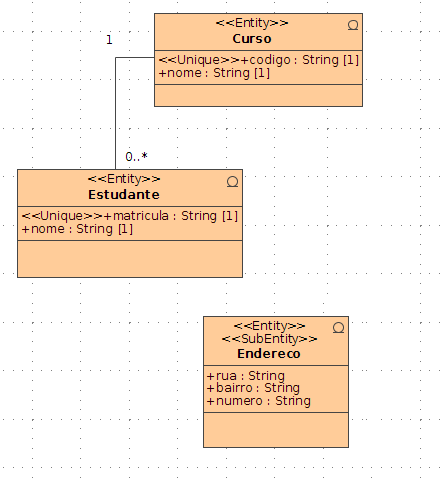
\includegraphics[width=290pt,height=300pt]{files/imgs/tutorial-mdarte-jsonb-0002.png}
	\caption{Classe Endereco com os estereótipos para a subentidade JSONB.}
	\label{camada_dominio_endereco_estereotipos}
\end{figure}

A maneira de expressar que uma determinada subentidade JSONB é faz parte de uma
determinada entidade é através de uma associação. É importante lembrar que cada
subentidade só pode ser parte de uma única entidade, por tanto deve ter um único
relacionamento.

A subentidade JSONB do MDArte permite salvar e manter tanto um único objeto JSON
como um array destes objetos, sendo isso definido de acordo com a
multiplicidade definida nos relacionamentos. A seguir veremos exemplos de como
modelar ambas as situações.

Começaremos modelando o caso em que a entidade possui um campo JSONB que contém
um único objeto da subentidade JSONB. Como já foi dito, isso é definido por meio
de uma associação e sua multiplicidade. Modelaremos então uma associação entre a
entidade e a nossa subentidade JSONB, neste exemplo, entre Estudante e Endereco,
colocando multiplicidade 1 para ambas as entidades. O modelo ficará da seguinte
forma:

\begin{figure}[H]
	\centering
	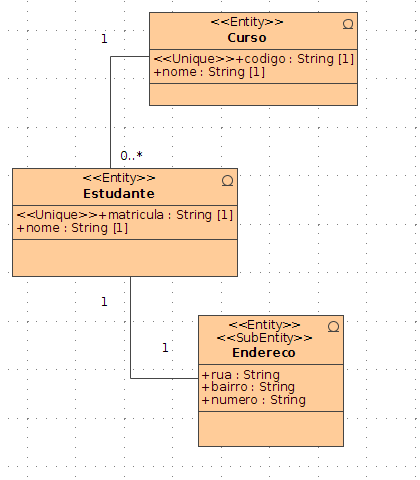
\includegraphics[width=290pt,height=320pt]{files/imgs/tutorial-mdarte-jsonb-0000.png}
	\caption{Modelando o Endereco como objeto simples pertencente à classe
	Estudante.}
	\label{camada_dominio_endereco_estereotipos}
\end{figure}

Modelaremos agora, alternativamente, o caso em que a entidade possui em si um
campo JSONB com um array de objetos do tipo da subentidade JSONB. Para tal,
modelaremos também uma associação entre as classes anteriormente citadas,
mudanddiferindo somente na multiplicidade referente à classe que mapeia a
subentidade, que neste caso deve ser \texttt{0\ldots*} ou \texttt{*}. O modelo
ficará como na imagem:

\begin{figure}[H]
	\centering
	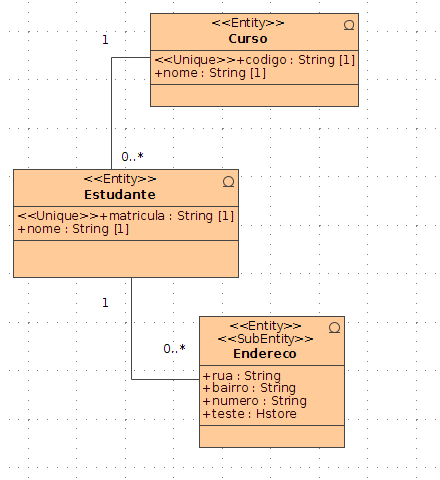
\includegraphics[width=290pt,height=320pt]{files/imgs/tutorial-mdarte-jsonb-0001.png}
	\caption{Modelando o Endereco como array de objetos pertencentes à
	classe Estudante.}
	\label{camada_dominio_endereco_estereotipos}
\end{figure}

Feita a modelagem conveniente à implementação que se está fazendo, vá na raiz do
projeto e rode o comando \texttt{maven}.

\subsection{Código gerado para a subentidade JSONB}
Nesta subseção veremos o código gerado para suportar o uso da subentidade JSONB
e a sua apropriada implementação e utilização. Para cada classe marcada com os
estereótipos \texttt{«Entity»} e \texttt{«SubEntity»}, o \texttt{MDArte} gera
as classes \texttt{<nomeDaSubentidade>.java} e
\texttt{<nomeDaSubentidade>Impl.java}, sendo, respectivamente, uma classe
abstrata, contendo os métodos de acesso e modificação dos dados da subentidade,
bem como os métodos modelados para a classe como métodos abstratos, e uma classe
que estende a primeira, funcionando como ponto de implementação para o métodos
modelados bem como qualquer outro código adicionado manualmente à subentidade.

A classe abstrata é gerada com os seguintes métodos:
\begin{itemize}
  \item Construtor sem parâmetro - Retorna uma instância da classe com todos os
  seus atributos tendo valor nulo;
  \item Construtor recebendo Map<String,String> por parâmetro - Retorna uma
  instância da classe inicializando seus atributos com os valores do Map
  correspondentes a seus respectivos nomes. Por exemplo, um atributo chamado
  `nome` receberia o valor relativo à chave 'nome' do Map. Todos os casts e
  conversões da String retornada pelo Map para o tipo do atributo são resolvidos
  pelo próprio construtor;
  \item public String toJson() - Retorna um JSON referente à instância da
  subentidade que o invoca;
  \item public <nomeDaSubentidade> clone - Retorna um clone da instância da
  subentidade que o invoca, ou seja, uma nova instância do objeto que no entanto
  contém todos os campos com o valor semelhante ao da instância que invocou tal
  método.
  \item Getters e Setters para cada atributo - Métodos usados para acessar e
  alterar os valores do atributos da instância da subentidade.
\end{itemize}

A classe de implementação é gerada somente com construtores que suportem a
extensão dos construtores da superclasse, ficando todo o restante da sua
implementação por conta do desenvolvedor.

\subsection{Codigo gerado na classe que contém a subentidade JSONB}
No caso de uma multiplicidade um para um na modelagem da associação, a classe da
entidade que contém a subentidade JSONB, terá como atributo uma instância da
classe referente à subentidade e métodos de get e set para acesso e alteração do
conteúdo da classe. Vale ressaltar que o método de set aceita tanto uma
instância da própria classe, ou um Map com os valores que seja deseja atribuir a
cada atributo relacionado à uma chave que corresponde a seu nome.

Caso contrário, a classe da entidade que contém a subentidade JSONB, terá um
ArrayList de objetos do tipo da classe que representa a subentidade. Na classe
da entidade o campo será gerado com o tipo ArrayList, e com o nome no plural, e
serão gerados os seguintes métodos para acessar e alterar os valores do
ArrayList:

\begin{itemize}
  \item getter - Retorna um clone da instância do ArrayList de subentidades
  contido na classe da entidade;
  \item setter - Recebe uma ArrayList por parâmetro, e cria uma nova lista
  contendo subentidades com valores semelhantes aos da ArrayList recebida;
  \item removeFrom<nomeDoAtributo> - Recebe um valor inteiro referente ao índice
  do ArraList que se deseja remover e retorna uma a subentidade removida da
  lista;
  \item addTo<nomeDoAtributo> - Método com duas assinaturas diferentes, podendo
  receber o índice do array onde adicionar e a subentidade a ser adicionada, ou
  somente a subentidade a ser adicionada, não tendo nenhum retorno.
\end{itemize}
